\pagestyle{simple}
\chapter{Projeto do Software}
\label{c.projeto}

O projeto do software é uma solução para a simulação da probabilidade de chuva de um determinado período para uma determinada cidade que tenha disponível dados históricos pluviométricos, de preferência maiores do que 20 anos.

O modelo em questão utiliza a Cadeia de Markov para gerar a probabilidade de ocorrência de chuva, para então determinar se o dia vai ser chuvoso ou seco. Para isso, deve ser analisado previamente um certo intervalo de dias anteriores ao dia a ser previsto. Como dito anteriormente, o trabalho adotou que se a precipitação pluviométrica de certo dia for maior ou igual a 0, então ele é considerado chuvoso. Caso contrário, é considerado seco.

A implementação em MATLAB é possível devido a facilidade de trabalho com vetores e matrizes que a ferramenta proporciona. Dando como \emph{input} as variáveis da tabela, cada uma organizada dentro de um vetor, foi viável a elaboração de um \emph{script} para gerar simular dias chuvosos e secos de um ano inteiro.

A cidade analisada foi Bauru, do estado de São Paulo, que tem disponível dados históricos desde 2002 através da Estacão Automática A705, latitude -22,358052 e longitude -49,028877. O ano simulado foi 2021 para que seja possível realizar uma comparação de resultados no final, a fim de verificar a precisão da simulação realizada neste trabalho.
\section{Especificação}
\label{s.especificacao}

Para realizar a simulação, com base no modelo analisado ~\cite{artigo_modelo}, é necessário efetuar um processo de geração das séries de dias secos e chuvosos através da comparação das probabilidades condicionais \emph{P(C|S)} e \emph{P(C|C)} com um número aleatório \emph{x} entre 0 e 1. O processo é inicializado em qualquer dia do mês simulado, desta forma, a definição do estado inicial (seco ou chuvoso) do dia anterior é obtida a partir de uma fonte meteorológica confiável. Para os demais dias, é feito da seguinte maneira:

\begin{enumerate}
  \item verifica se o dia anterior foi chuvoso ou seco. Nesse trabalho, um dia é considerado chuvoso quando a sua precipitação diária for maior do que 0mm;
  \item se o dia anterior for seco, gera-se um número aleatório \emph{x} entre 0 e 1, e o compara com a probabilidade condicional P(C|S) gerada para o dia atual analisado. Já se o dia anterior foi chuvoso, compara-se o número aleatório \emph{x} com a probabilidade condicional P(C|C) obtida para o dia atual analisado. Essa comparação é feita da seguinte forma:
  \begin{enumerate}[label=(\alph*)]
   \item se x $\leq$ P(C|S) ou P(C|C), o estado do dia atual é considerado chuvoso; 
   \item se x > P(C|S) ou P(C|C), o estado do dia atual é considerado seco.
  \end{enumerate}
\end{enumerate}

As probabilidades condicionais são definidas com base na Cadeia de Markov, com suas fórmulas descritas abaixo:

\[
    P(C|S)=\frac{N(C|S)}{N(C|S)+N(C|S)}=\frac{N(C|S)}{N(S)}
\]
\[
    P(C|C)=\frac{N(C|C)}{N(S|C)+N(C|C)}=\frac{N(C|C)}{N(C)}
\]

\section{Tecnologias Pesquisadas e Escolhidas}
\label{s.tecnologias}

Existem diversas tecnologias que são capazes de realizar a simulação pluviométrica de maneira satisfatória. De todas as analisadas, a ferramenta escolhida foi o MATLAB, uma linguagem de programação de alta performance voltada para o cálculo numérico.

\subsection{MATLAB}
\label{ss.matlab}

Para um projeto que envolve muitos cálculos numéricos e manipulações de extensas matrizes e vetores, o software MATLAB é líder no segmento ~\cite{matlab}. Trata-se de um software robusto que consegue resolver muitos problemas em um tempo muito menor de programação quando comparado a outras linguagens de programação.
A versão escolhida para realizar o trabalho foi a R2021a, lançada em março de 2021, 
porém existem muitas outras versões desde o ano de 1984.
Trata-se de um software proprietário pago, mas existem licenças exclusivas para estudantes de universidade.

\begin{figure}[H]
    \caption{\small Demonstração de sintaxe na IDE do MATLAB.}
	\centering
	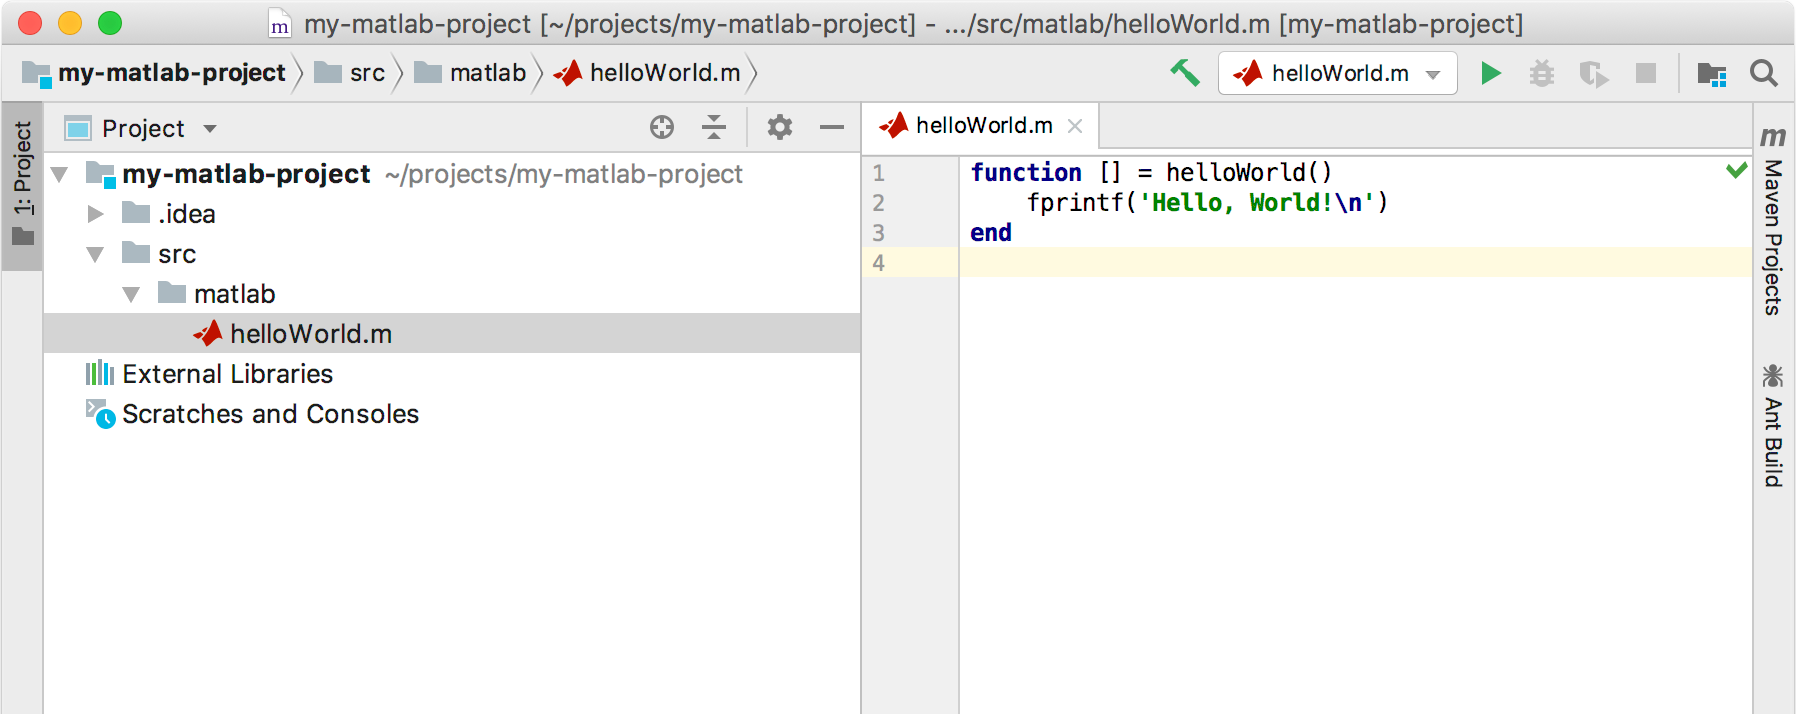
\includegraphics[width=\textwidth]{figs/matlab-syntax.png}
	\label{f.matlab-syntax}
	\legend{\small Fonte: \cite{matlab-jetbrains}.}
\end{figure}

\subsection{Mathematica}
\label{ss.mathematica}

É outro programa que permite resolver problemas matemáticos com certa facilidade, utilizando de várias bibliotecas de programação para auxiliar na resolução de problemas de ciências exatas.
O sistema é utilizado em muitas áreas da computação, como redes neurais, aprendizado de máquina, processamento de imagens, geometria, ciência de dados, visualizações e diversas outras ~\cite{mathematica}.

\begin{figure}[H]
    \caption{\small Demonstração de sintaxe na IDE do Mathematica.}
	\centering
	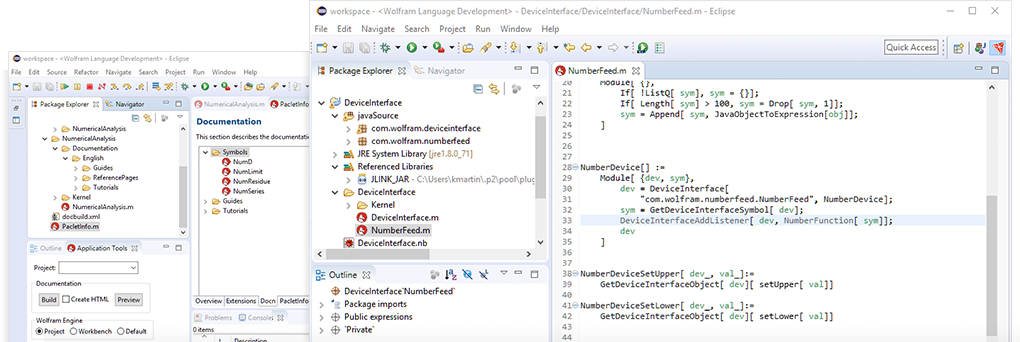
\includegraphics[width=\textwidth]{figs/mathematica-ide.png}
	\label{f.matlab-syntax}
	\legend{\small Fonte: \cite{mathematica}.}
\end{figure}

\subsection{GNU Octave}
\label{ss.gnu}

Em termos de compatibilidade e capacidade computacional, o GNU Octave é considerado a melhor alternativa do MATLAB ~\cite{matlab-alts}. A maioria dos projetos desenvolvidos para o MATLAB também conseguem ser executados no Octave. Além disso, ele roda em qualquer sistema operacional sem nenhuma modificação. 

Ele pode lidar com grandes sintaxes matemáticas e tem ferramentas de plotagem e visualização. Além disso, é um software de código aberto e foi desenvolvido principalmente para cálculos numéricos lineares e não lineares complexos. Ele pode executar trabalhos interativos e em lote e tem compatibilidade com \emph{scripts} MATLAB e outros escritos em Java, C++ ou Fortran.

\begin{figure}[H]
	\caption{\small Demonstração de sintaxe na IDE do GNU Octave.}
	\centering
	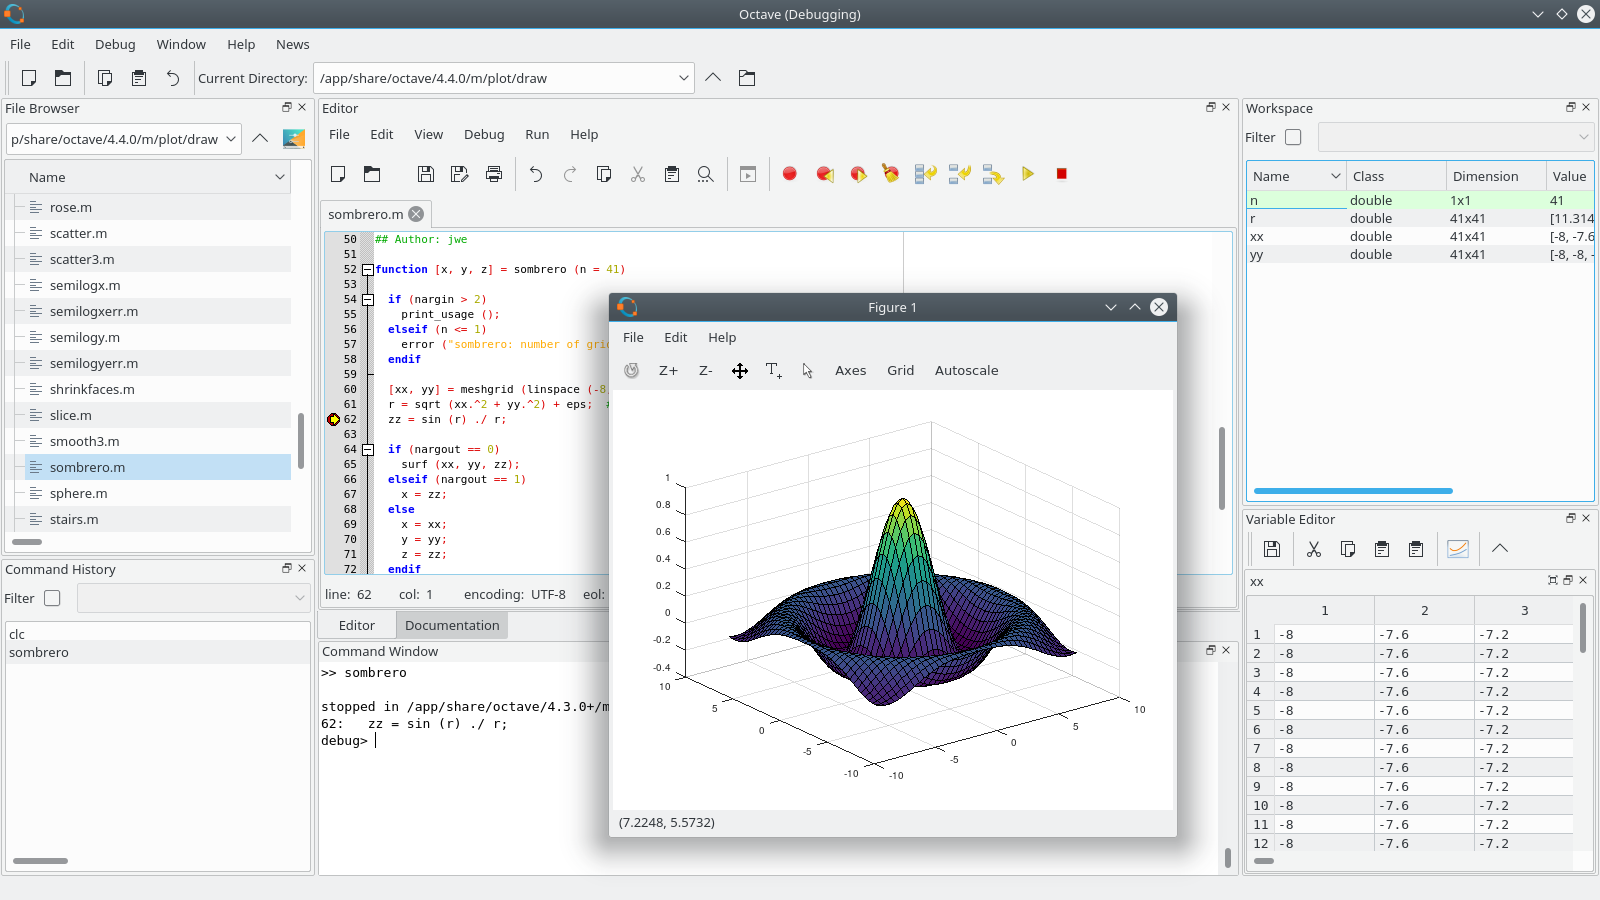
\includegraphics[width=\textwidth]{figs/octave-ide.png}
	\label{f.matlab-syntax}
	\legend{\small Fonte: \cite{octave-ide}.}
\end{figure}